\tableofcontents
\clearpage

\section*{Введение}

\textbf{Цель работы:} ознакомление с принципами функционирования, построения и особенностями архитектуры суперскалярных конвейерных микропроцессоров. Дополнительной целью работы является знакомство с принципами проектирования и верификации сложных цифровых устройств с использованием языка описания аппаратуры SystemVerilog и ПЛИС.

Для достижения поставленных целей в настоящей лабораторной работе
используется синтезируемое описание микропроцессорного ядра
Taiga\footnote{https://gitlab.com/sfu-rcl/Taiga, авторы - Eric Matthews,  Lesley Shannon},
реализующего систему команд RV32I семейства RISC-V. Данное описание выполнено на языке описания аппаратуры SystemVerilog.

В ходе лабораторной работы используется средство моделирования Modelsim для моделирования работы исследуемого микропроцессора в процессе выполнения программы и наблюдения формы внутренних сигналов.

Все задания выполняются в соответствии с вариантом №10.

\section{Задание №1}
\subsection{Текст программы по индивидуальному варианту}

\begin{lstlisting}[label=programText,caption=Текст программы по индивидуальному варианту]
        .section .text
		.globl _start;
		len = 8
		enroll = 4
		elem_sz = 4

_start:
		addi x20, x0, len/enroll
		la x1, _x
		add x31, x0, x0
lp:
		lw x2, 0(x1)
		lw x3, 4(x1) #!
		add x31, x31, x2
		add x31, x31, x3
		lw x4, 8(x1)
		lw x5, 12(x1)
		add x31, x31, x4
		add x31, x31, x5
		addi x1, x1, elem_sz*enroll
		addi x20, x20, -1
		bne x20, x0, lp
		addi x31, x31, 1
lp2: j lp2

		.section .data
_x:     .4byte 0x1
		.4byte 0x2
		.4byte 0x3
		.4byte 0x4
		.4byte 0x5
		.4byte 0x6
		.4byte 0x7
		.4byte 0x8
\end{lstlisting}

\subsection{Дизассемблерный листинг кода программы}
В результате выполнения компиляции был создан файл с расширением .hex, хранящий содержимое памяти команд и данных. В окне терминала отобразился дизассемблерный листинг, который приведен в листинге \ref{img:disassembler}.

\begin{lstlisting}[extendedchars=true, keepspaces=true, escapechar=\%, texcl=true, label=img:disassembler,caption=Дизассемблированная программа по варианту]
	SYMBOL TABLE:
	80000000 l    d  .text	00000000 .text
	80000044 l    d  .data	00000000 .data
	00000000 l    df *ABS*	00000000 myprog.o
	00000008 l       *ABS*	00000000 len
	00000004 l       *ABS*	00000000 enroll
	00000004 l       *ABS*	00000000 elem_sz
	80000044 l       .data	00000000 _x
	80000010 l       .text	00000000 lp
	80000040 l       .text	00000000 lp2
	80000000 g       .text	00000000 _start
	80000064 g       .data	00000000 _end
	
	Дизассемблирование раздела .text:
	
	80000000 <_start>:
	80000000:	00200a13          	addi	x20,x0,2
	80000004:	00000097          	auipc	x1,0x0
	80000008:	04008093          	addi	x1,x1,64 # 80000044 <\_x>
	8000000c:	00000fb3          	add	x31,x0,x0
	
	80000010 <lp>:
	80000010:	0000a103          	lw	x2,0(x1)
	80000014:	0040a183          	lw	x3,4(x1)
	80000018:	002f8fb3          	add	x31,x31,x2
	8000001c:	003f8fb3          	add	x31,x31,x3
	80000020:	0080a203          	lw	x4,8(x1)
	80000024:	00c0a283          	lw	x5,12(x1)
	80000028:	004f8fb3          	add	x31,x31,x4
	8000002c:	005f8fb3          	add	x31,x31,x5
	80000030:	01008093          	addi	x1,x1,16
	80000034:	fffa0a13          	addi	x20,x20,-1
	80000038:	fc0a1ce3          	bne	x20,x0,80000010 <lp>
	8000003c:	001f8f93          	addi	x31,x31,1
	
	80000040 <lp2>:
	80000040:	0000006f          	jal	x0,80000040 <lp2>
	
	Дизассемблирование раздела .data:
	
	80000044 <_x>:
	80000044:	0001                	c.addi	x0,0
	80000046:	0000                	c.unimp
	80000048:	0002                	c.slli64	x0
	8000004a:	0000                	c.unimp
	8000004c:	00000003          	lb	x0,0(x0) # 0 <elem\_sz-0x4>
	80000050:	0004                	.2byte	0x4
	80000052:	0000                	c.unimp
	80000054:	0005                	c.addi	x0,1
	80000056:	0000                	c.unimp
	80000058:	0006                	c.slli	x0,0x1
	8000005a:	0000                	c.unimp
	8000005c:	00000007          	.4byte	0x7
	80000060:	0008                	.2byte	0x8
	...
\end{lstlisting}

\subsection{Псевдокод, поясняющий работу программы}
На листинге \ref{pscode} приведен псевдокод, поясняющий работу программы.

\begin{lstlisting}[extendedchars=true, keepspaces=true, escapechar=\%, texcl=true, label=pscode,caption=Псевдокод\, поясняющий работу программы]
	#define len 8
	#define enroll 4
	#define elem\_sz 4
	int _x[] = {1, 2, 3, 4, 5, 6, 7, 8};
	
	void start(){
		int x20 = len/enroll;
		int *x1 = _x;
		int x_31 = 0;
		
		do
		{
			int x2 = x1[0];
			int x3 = x1[1];
			x31 += x2;
			x31 += x3;
			
			int x4 = x1[2];
			int x5 = x1[3];
			x31 += x4;
			x31 += x5;
			
			x1 += enroll;
			x20--;
		} while (x20 != x0)
		
		x31 += 1;
		
		while(1) {}
	}
\end{lstlisting}

Очевидно, что в регистре x31 после выполнения программы должно содержаться значение:
\begin{displaymath}
	x31 = \sum\limits_{i=1}^8{i} + 1 = 37.
\end{displaymath}
\newpage

\section{Задание №2}
В результате симуляции, был получен снимок экрана, содержащий временную диаграмму выполнения стадий выборки и диспетчеризации команды с адресом 80000030 (1 итерация). Снимок экрана приведен на рисунке \ref{fetch}.

\begin{figure}[h!p]
	\centering
	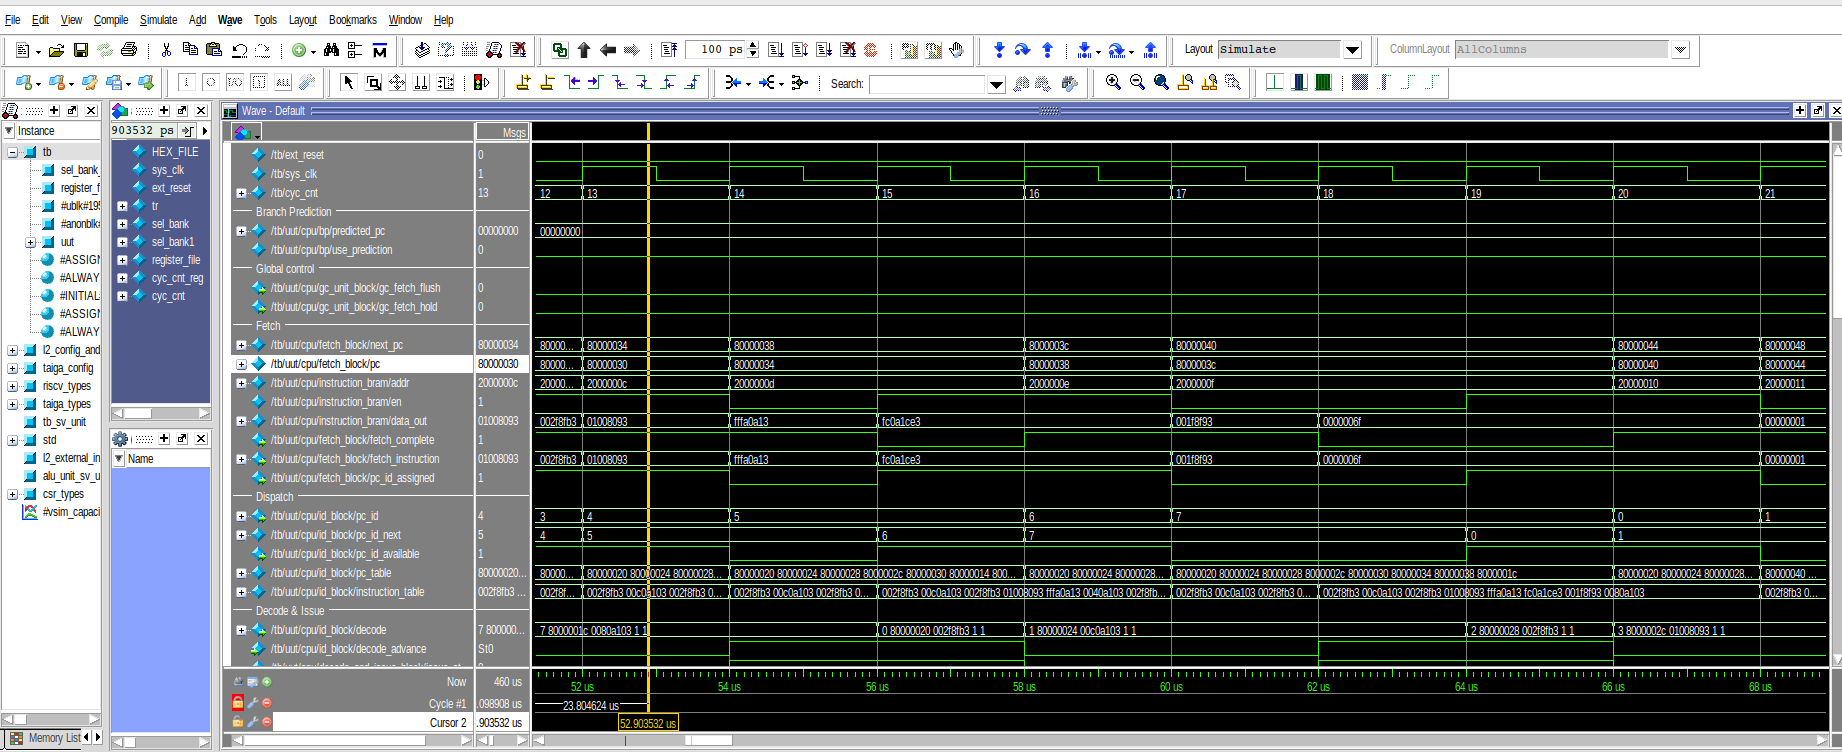
\includegraphics[width = \linewidth]{../img/fetch.png}
	\caption{Временная диаграмма выполнения стадий выборки и диспетчеризации команды с адресом 80000030 (1 итерация)}
	\label{fetch}
\end{figure}

\section{Задание №3}
В результате симуляции, был получен снимок экрана, содержащий временную диаграмму выполнения стадии декодирования и планирования на выполнение команды с адресом 80000010 (2 итерация). Снимок экрана приведен на рисунке \ref{decode}.

\begin{figure}[h!p]
	\centering
	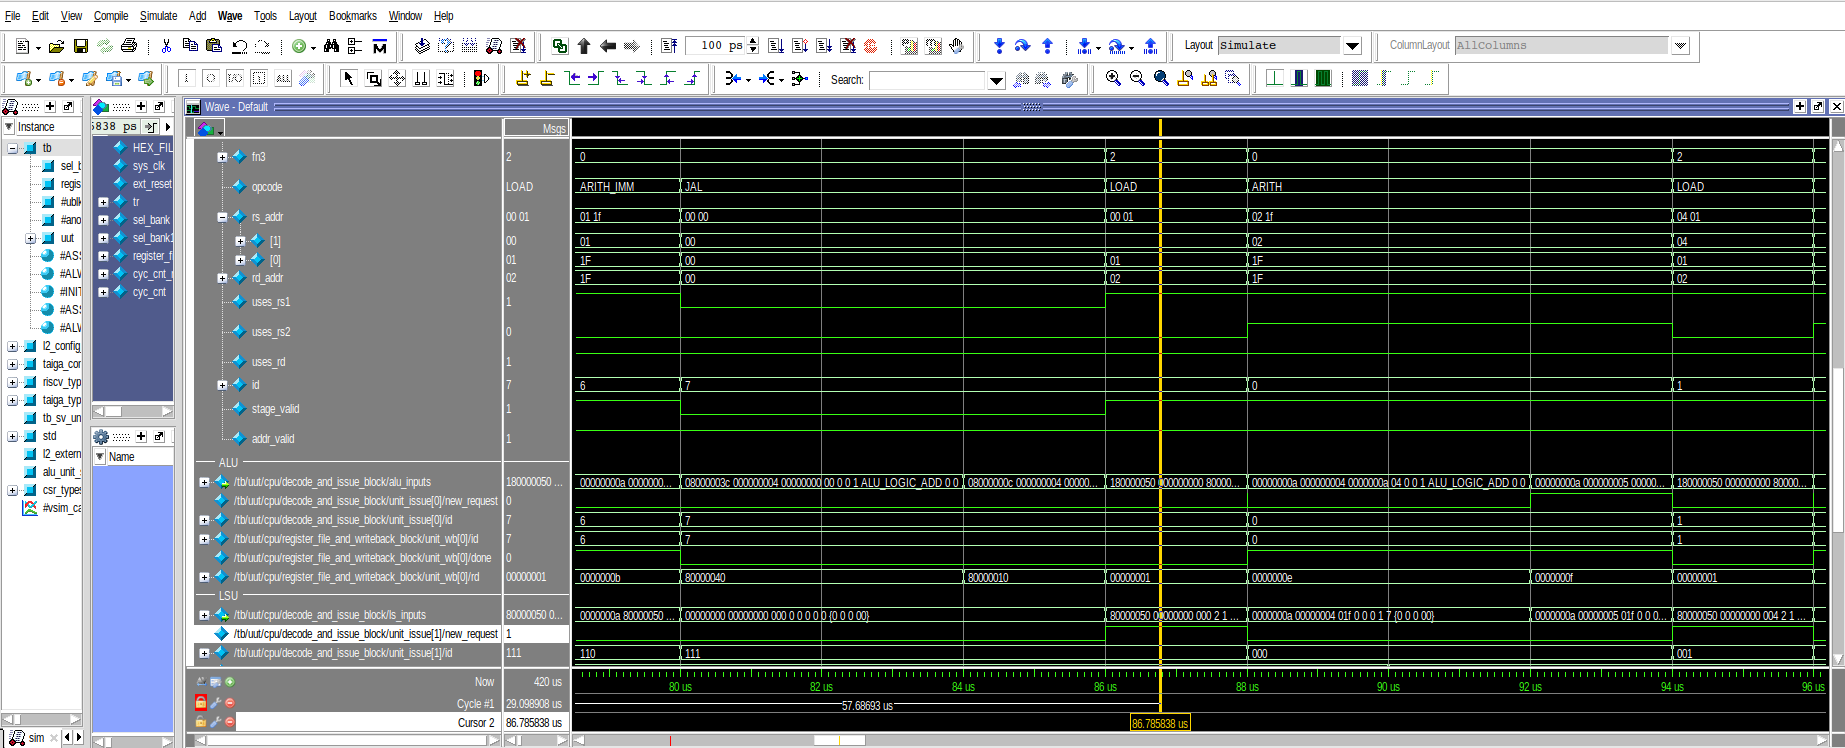
\includegraphics[width = \linewidth]{../img/decode.png}
	\caption{Временная диаграмма выполнения стадий декодирования и планитрования на выполнение команды с адресом 80000010 (2 итерация)}
	\label{decode}
\end{figure}

\section{Задание №4}
В результате симуляции, был получен снимок экрана, содержащий временную диаграмму стадии выполнения команды с адресом 80000024 (1 итерация). Снимок экрана приведен на рисунке \ref{exec}.

\begin{figure}[h!p]
	\centering
	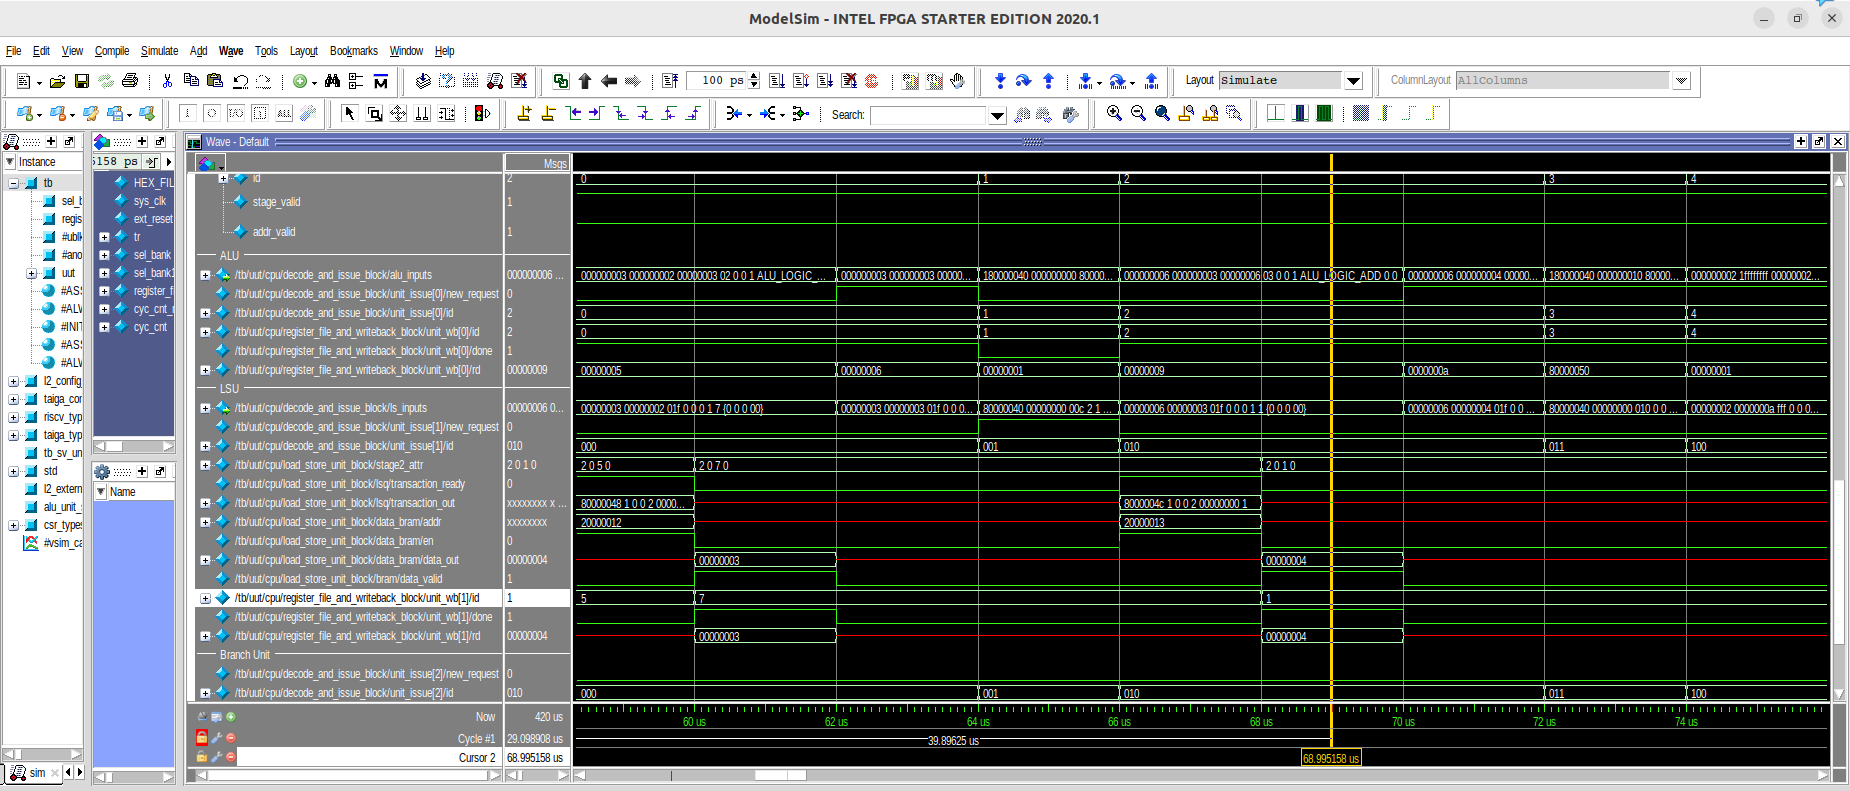
\includegraphics[width = \linewidth]{../img/exec.png}
	\caption{Временная диаграмма стадии выполнения команды с адресом 80000024 (1 итерация)}
	\label{exec}
\end{figure}

\section{Задание №5}

Значение регистра $x31$ в конце выполнения программы равно $25h = 37$, как и предполагалось ранее. Скриншот представлен на рисунке \ref{resx31}.

\begin{figure}[h!p]
	\centering
	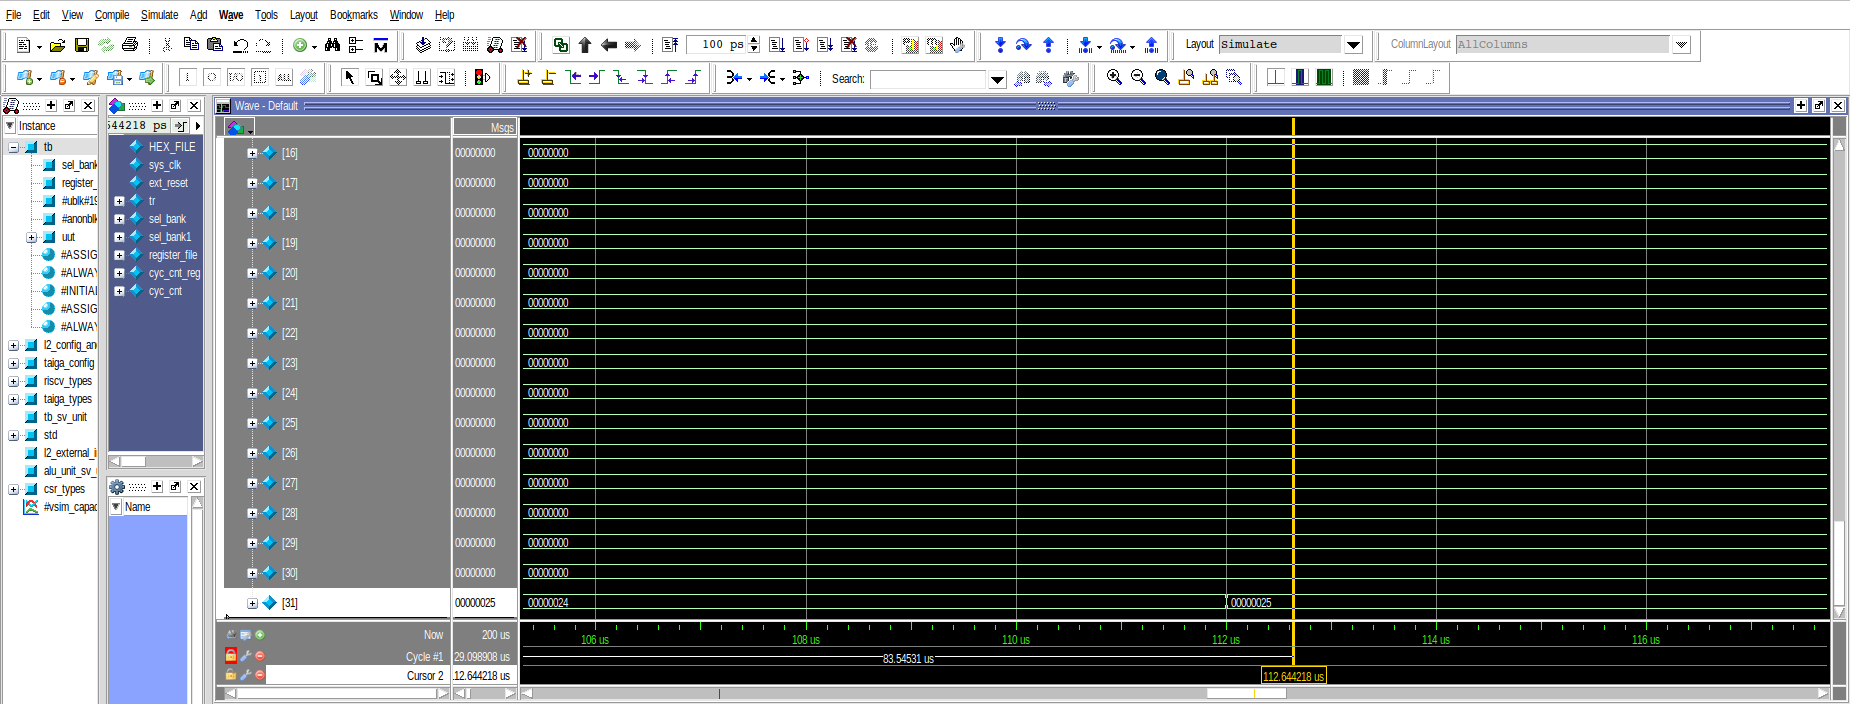
\includegraphics[width = \linewidth]{../img/resx31.png}
	\caption{Значение регистра x31 в конце выполнения программы}
	\label{resx31}
\end{figure}

На рисунках \ref{fid2} --- \ref{lsu2} представлены временные диаграммы сигналов, соответствующих всем стадиям выполнения команды, обозначенной в тексте программы символом \#!: команда lw x3,4(x1), имеющая код 0040a183 и адрес 80000014.

\begin{figure}[h!p]
	\centering
	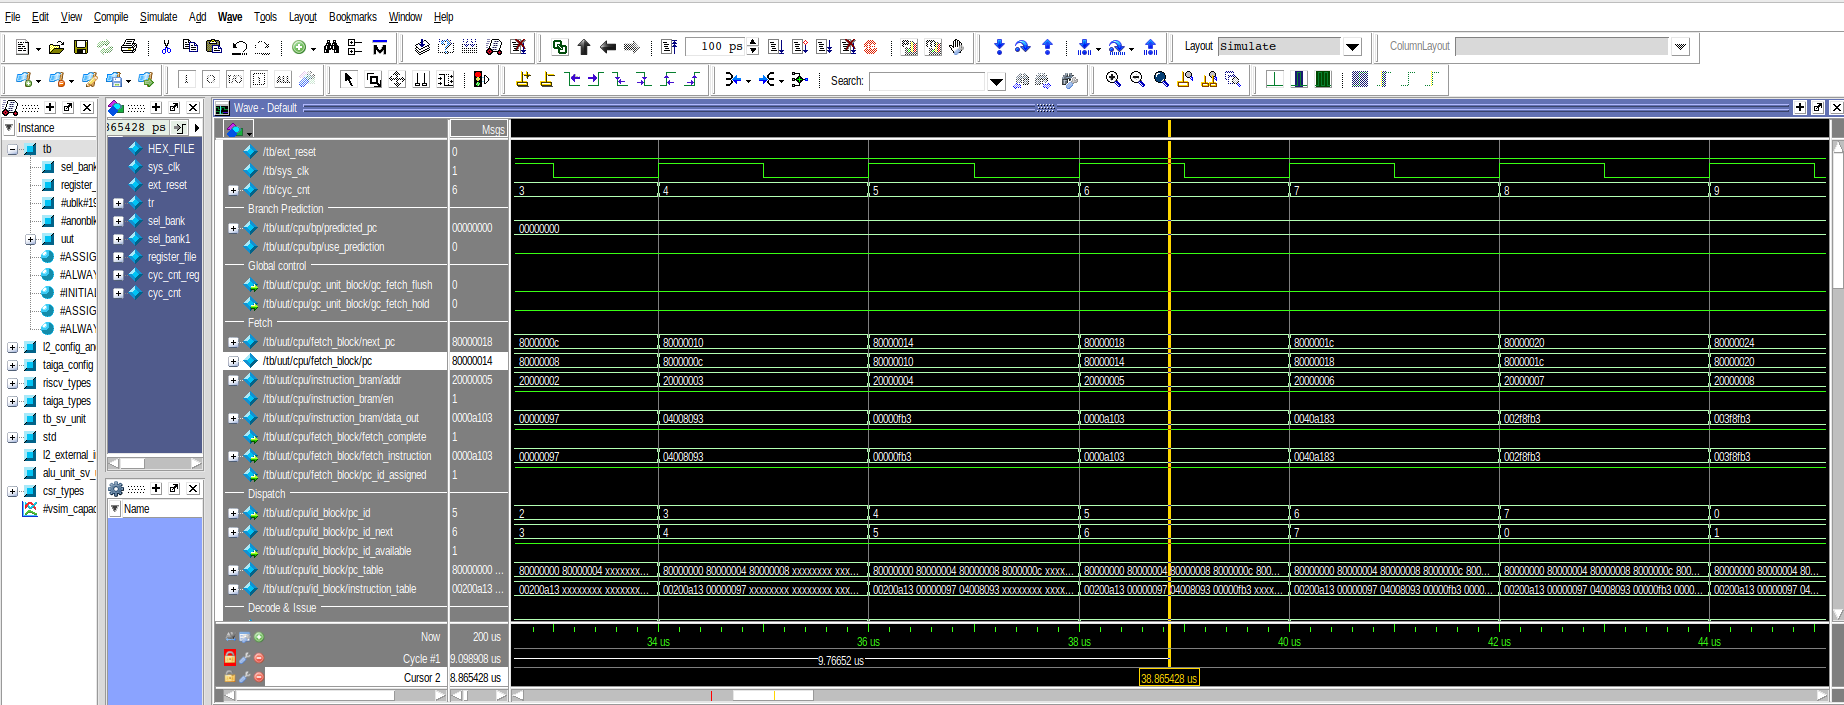
\includegraphics[width = \linewidth]{../img/fid2.png}
	\caption{Стадии выборки и диспетчеризации команды lw x3,4(x1)}
	\label{fid2}
\end{figure}

\begin{figure}[h!p]
	\centering
	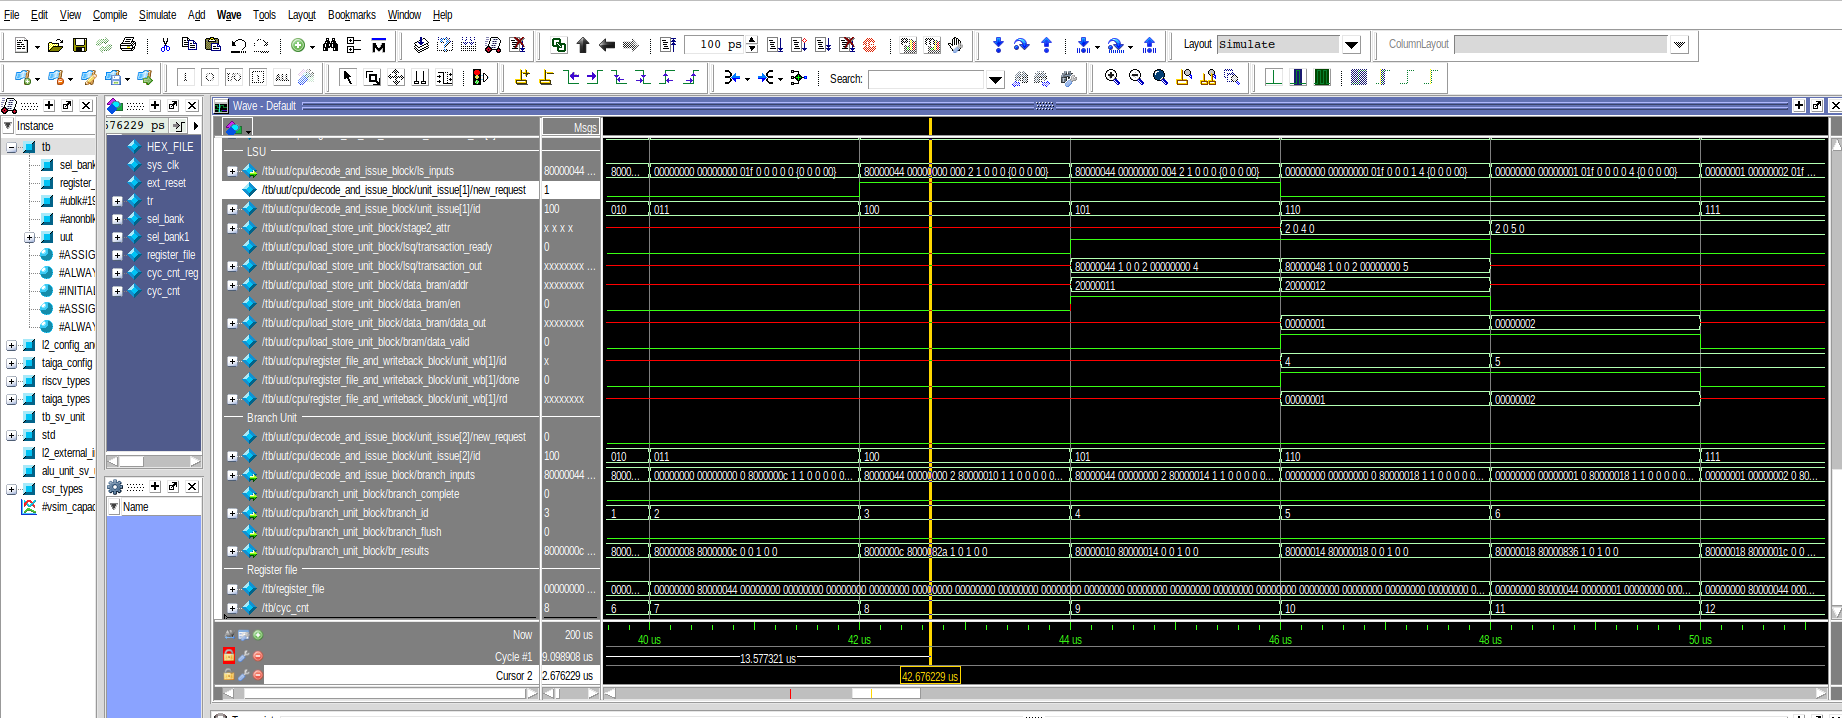
\includegraphics[width = \linewidth]{../img/decode2.png}
	\caption{Стадия декодирования команды lw x3,4(x1)}
	\label{decode2}
\end{figure}

\begin{figure}[h!p]
	\centering
	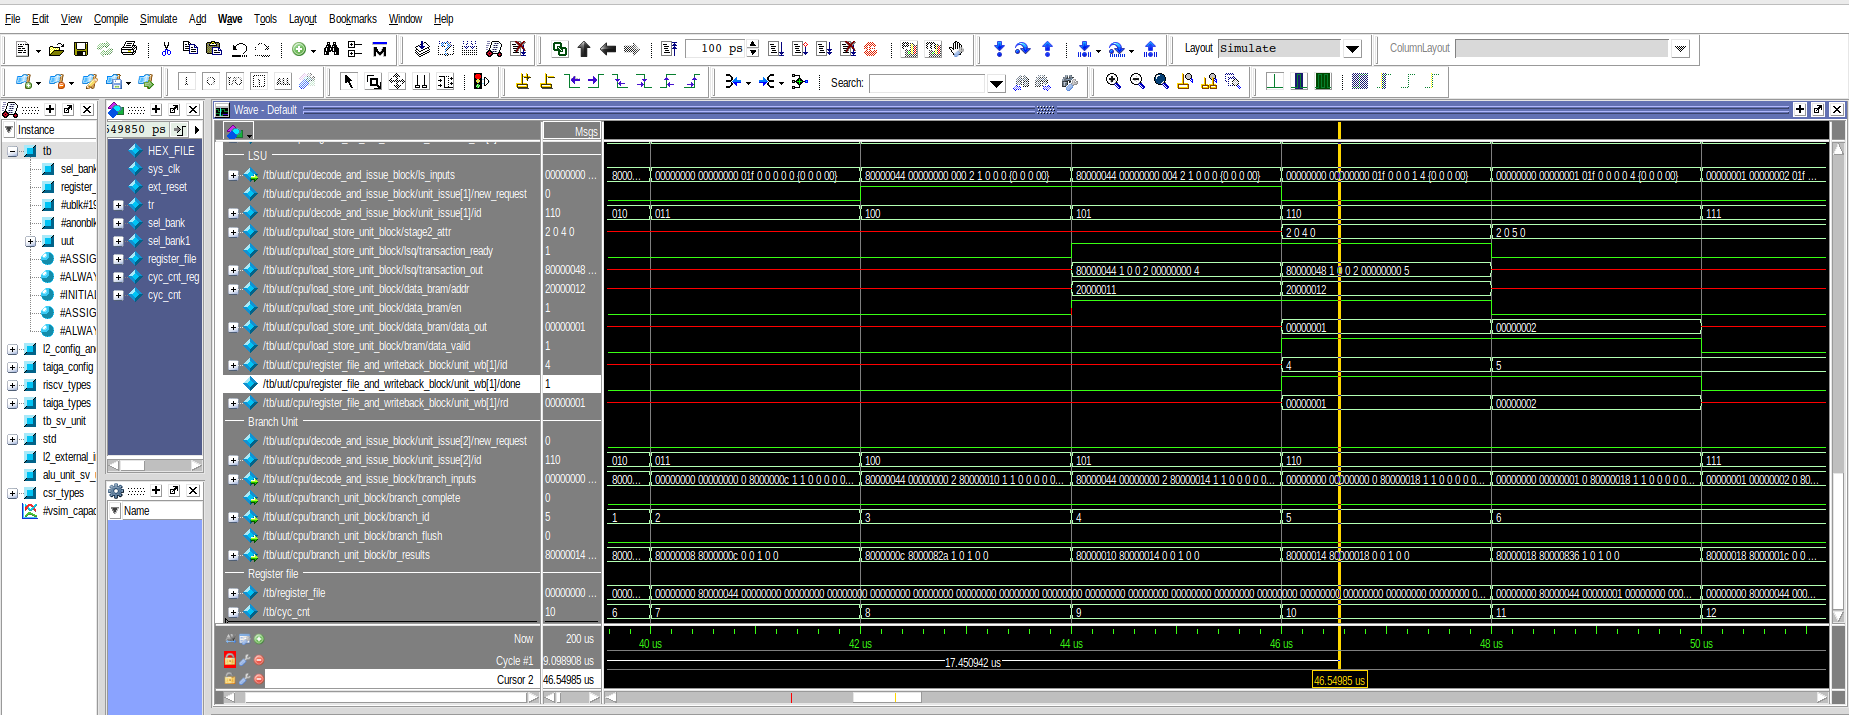
\includegraphics[width = \linewidth]{../img/lsu2.png}
	\caption{Стадия выполнения команды lw x3,4(x1)}
	\label{lsu2}
\end{figure}

Трасса неоптимизированной программы представлена на рисунке \ref{trace1}.

\begin{figure}[h!p]
	\centering
	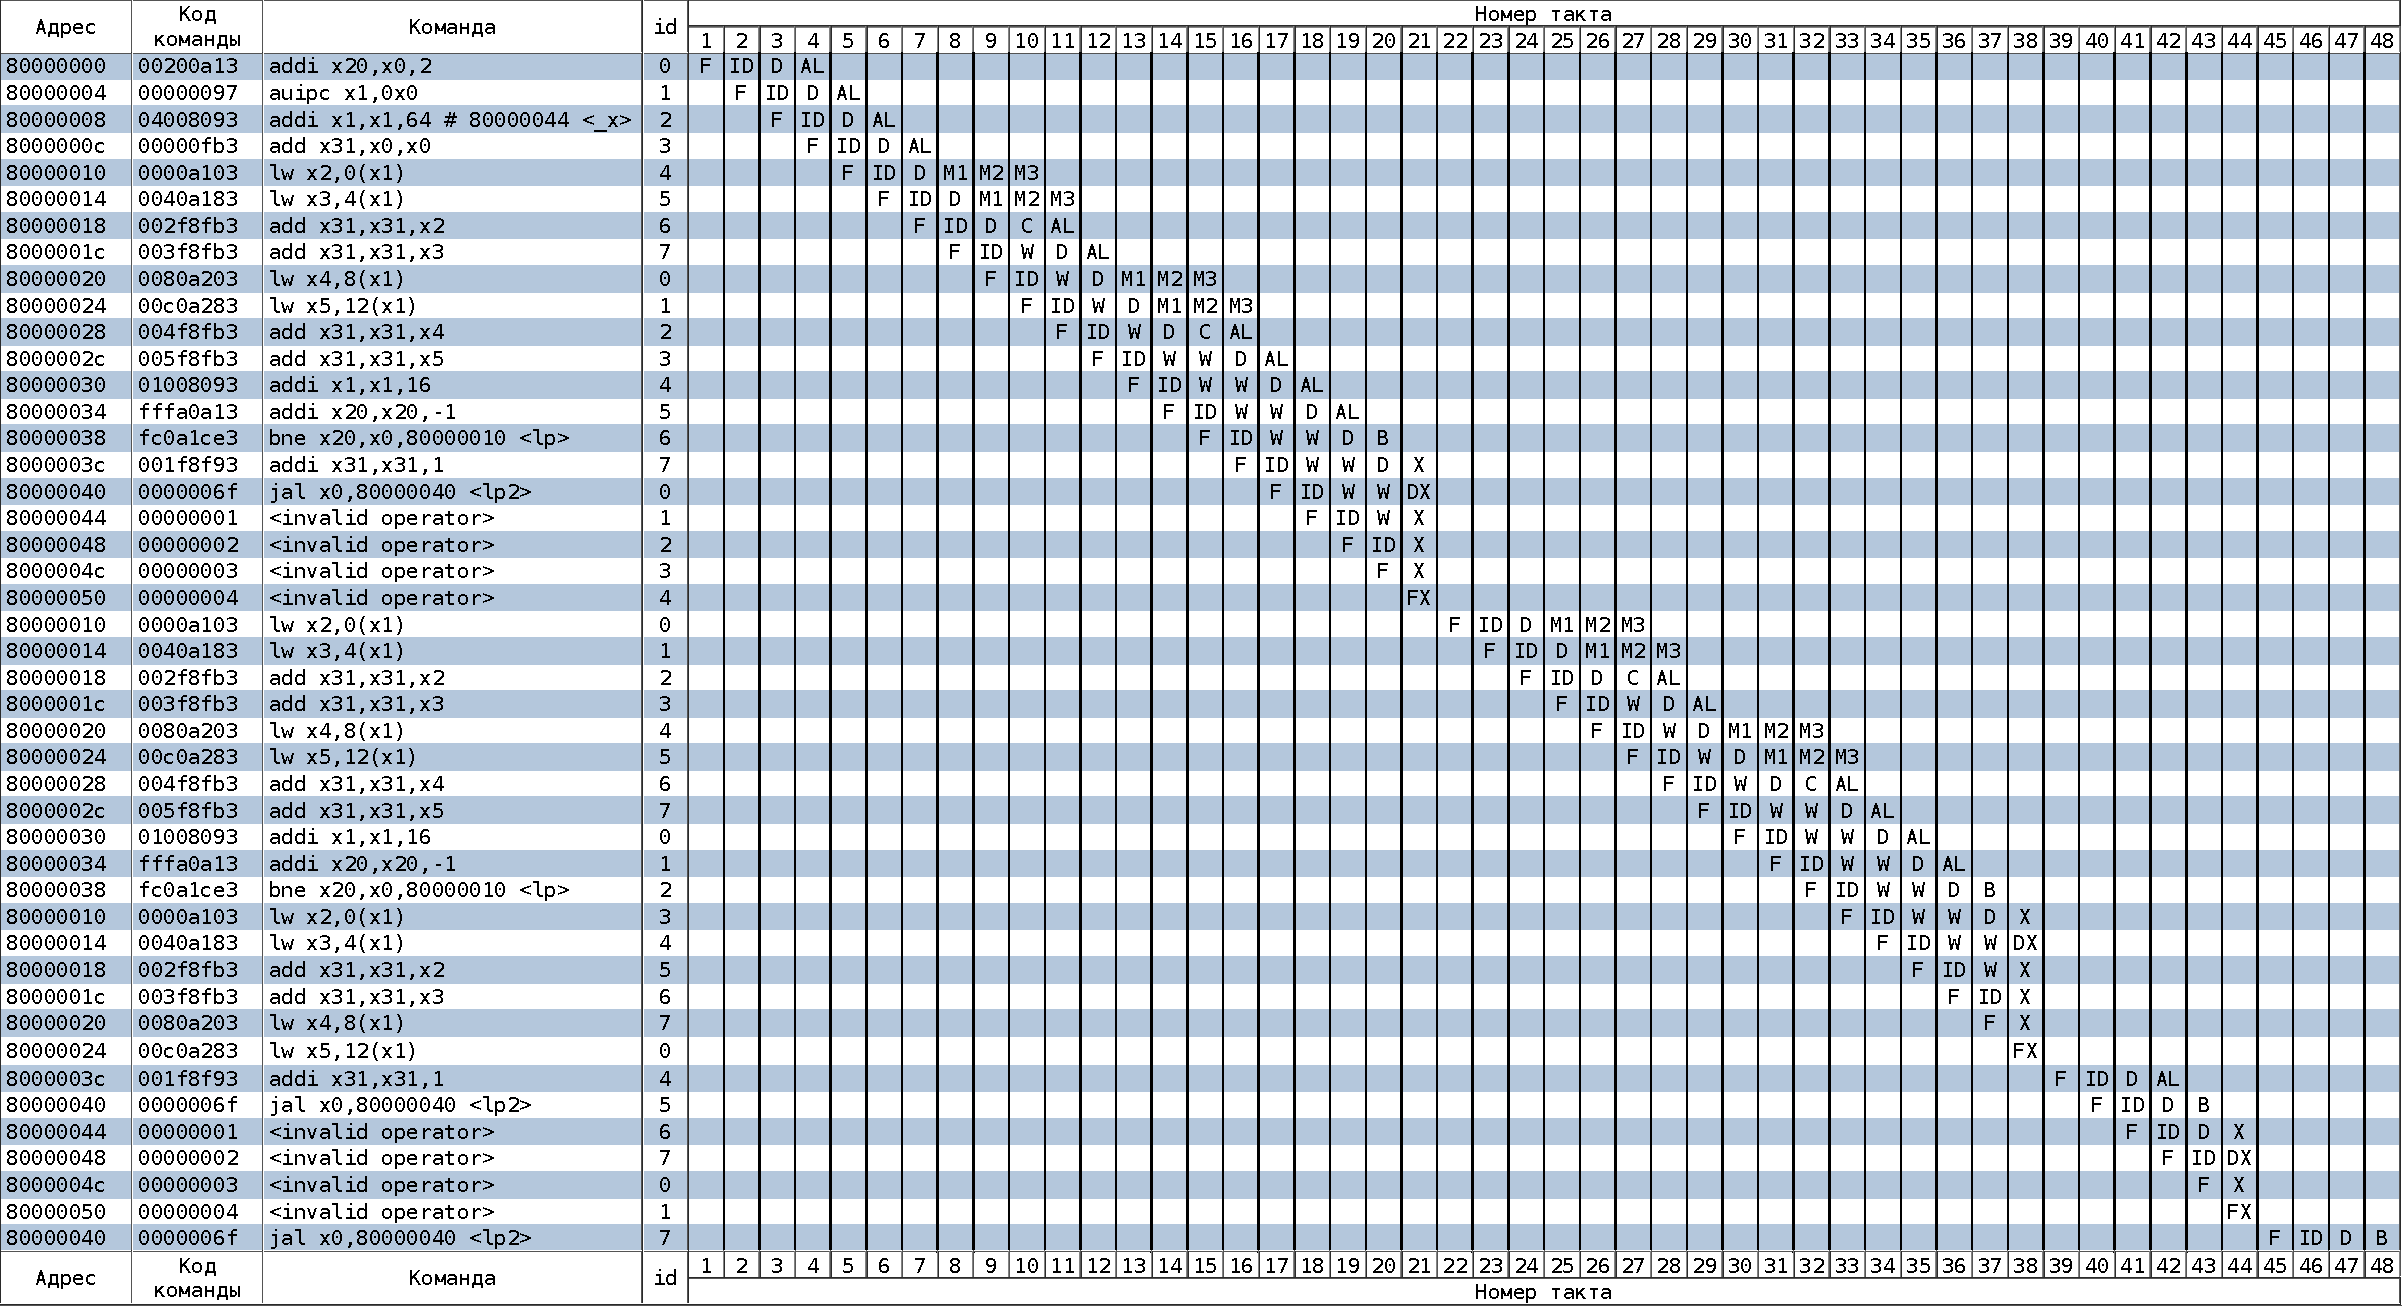
\includegraphics[width = \linewidth]{../img/trace1.pdf}
	\caption{Трасса работы неоптимизированной программы}
	\label{trace1}
\end{figure}

Конфликты возникают при выполнении команды \textit{add} после команды \textit{lw}. Для оптимизации (уменьшения числа конфликтов) перенесем все команды \textit{lw} так, чтобы все они выполнялись раньше команд \textit{add}.

Текст полученной программы представлен в листинге \ref{lst:opt}, а ее дизассемблерный листинг --- в листинге \ref{lst:opthex}

\begin{lstlisting}[label=lst:opt,caption=Текст оптимизированной программы]
	.section .text
	.globl _start;
	len = 8
	enroll = 4
	elem_sz = 4
	
	_start:
	addi x20, x0, len/enroll
	la x1, _x
	add x31, x0, x0
	lp:
	lw x2, 0(x1)
	lw x3, 4(x1) #!
	lw x4, 8(x1)
	lw x5, 12(x1)
	add x31, x31, x2
	add x31, x31, x3
	add x31, x31, x4
	add x31, x31, x5
	addi x1, x1, elem_sz*enroll
	addi x20, x20, -1
	bne x20, x0, lp
	addi x31, x31, 1
	lp2: j lp2
	
	.section .data
	_x:     .4byte 0x1
	.4byte 0x2
	.4byte 0x3
	.4byte 0x4
	.4byte 0x5
	.4byte 0x6
	.4byte 0x7
	.4byte 0x8
\end{lstlisting}

\begin{lstlisting}[label=lst:opthex,caption=Дизассемблированная оптимизированная программа]
	SYMBOL TABLE:
	80000000 l    d  .text	00000000 .text
	80000044 l    d  .data	00000000 .data
	00000000 l    df *ABS*	00000000 optcode.o
	00000008 l       *ABS*	00000000 len
	00000004 l       *ABS*	00000000 enroll
	00000004 l       *ABS*	00000000 elem_sz
	80000044 l       .data	00000000 _x
	80000010 l       .text	00000000 lp
	80000040 l       .text	00000000 lp2
	80000000 g       .text	00000000 _start
	80000064 g       .data	00000000 _end
	
	
	
	Дизассемблирование раздела .text:
	
	80000000 <_start>:
	80000000:	00200a13          	addi	x20,x0,2
	80000004:	00000097          	auipc	x1,0x0
	80000008:	04008093          	addi	x1,x1,64 # 80000044 <_x>
	8000000c:	00000fb3          	add	x31,x0,x0
	
	80000010 <lp>:
	80000010:	0000a103          	lw	x2,0(x1)
	80000014:	0040a183          	lw	x3,4(x1)
	80000018:	0080a203          	lw	x4,8(x1)
	8000001c:	00c0a283          	lw	x5,12(x1)
	80000020:	002f8fb3          	add	x31,x31,x2
	80000024:	003f8fb3          	add	x31,x31,x3
	80000028:	004f8fb3          	add	x31,x31,x4
	8000002c:	005f8fb3          	add	x31,x31,x5
	80000030:	01008093          	addi	x1,x1,16
	80000034:	fffa0a13          	addi	x20,x20,-1
	80000038:	fc0a1ce3          	bne	x20,x0,80000010 <lp>
	8000003c:	001f8f93          	addi	x31,x31,1
	
	80000040 <lp2>:
	80000040:	0000006f          	jal	x0,80000040 <lp2>
	
	Дизассемблирование раздела .data:
	
	80000044 <_x>:
	80000044:	0001                	c.addi	x0,0
	80000046:	0000                	c.unimp
	80000048:	0002                	c.slli64	x0
	8000004a:	0000                	c.unimp
	8000004c:	00000003          	lb	x0,0(x0) # 0 <elem_sz-0x4>
	80000050:	0004                	.2byte	0x4
	80000052:	0000                	c.unimp
	80000054:	0005                	c.addi	x0,1
	80000056:	0000                	c.unimp
	80000058:	0006                	c.slli	x0,0x1
	8000005a:	0000                	c.unimp
	8000005c:	00000007          	.4byte	0x7
	80000060:	0008                	.2byte	0x8
	...
\end{lstlisting}

На рисунке \ref{trace2} представлена трасса оптимизированной программы.

\begin{figure}[h!p]
	\centering
	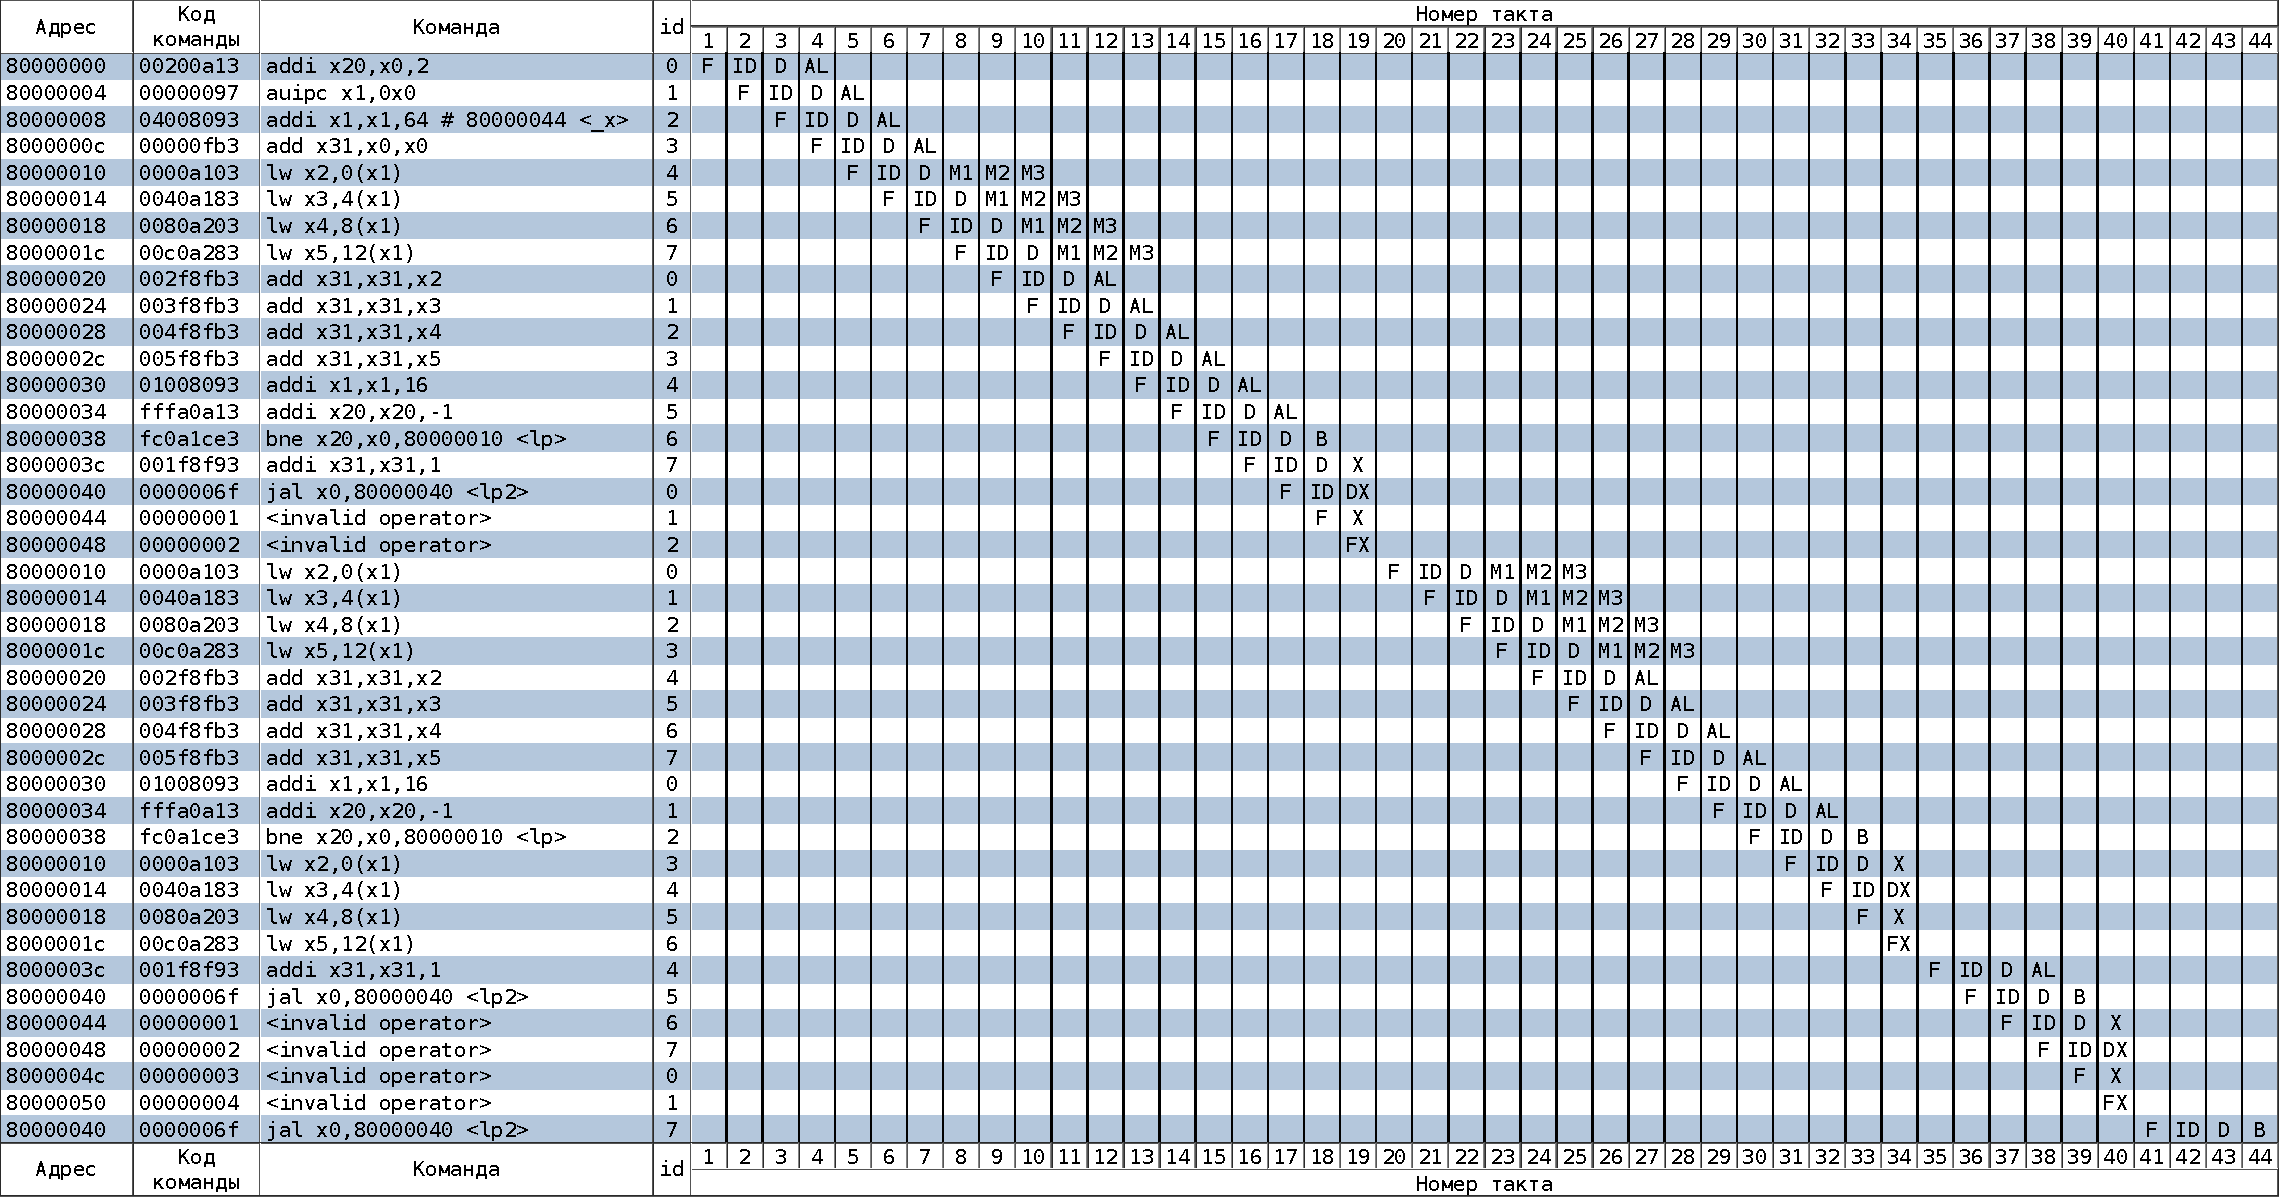
\includegraphics[width = \linewidth]{../img/trace2.pdf}
	\caption{Трасса работы оптимизированной программы}
	\label{trace2}
\end{figure}

Благодаря оптимизации программы получилось избавиться от конфликтов, а значит сократить время выполнения.
